% Generated by src/tools/c-f17-where-squares.py from evidence/figures/c-f17-where-squares.csv. Do not edit.
\node[anchor=north west, inner sep=0] at (0,0.0000) {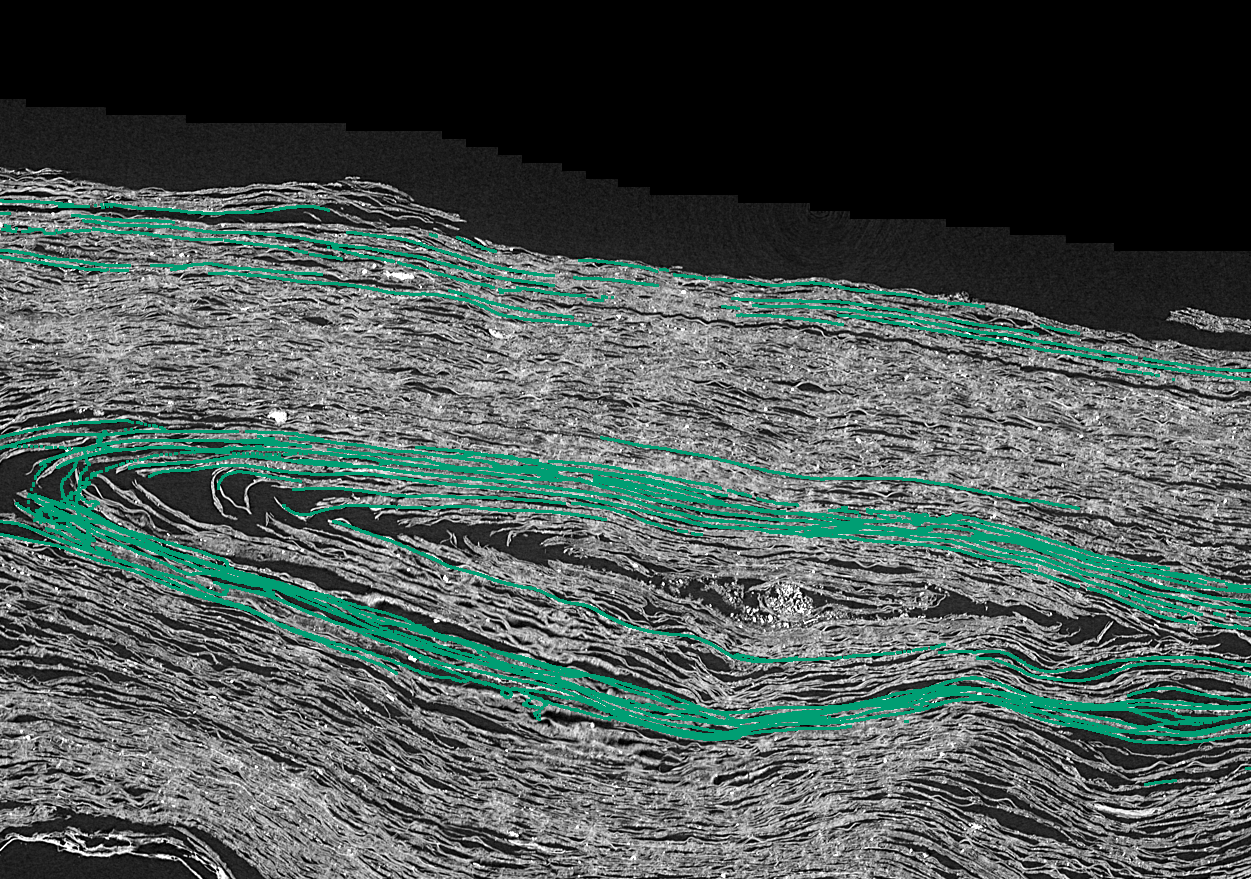
\includegraphics[width=8.6000cm]{../paper/figures/assets/c-f17-where-squares-slice-zoom.png}};
\node[hf] (m0) at (6.311,-4.704) {};
\node[hf] (m1) at (6.562,-4.819) {};
\node[hf] (m2) at (6.989,-3.341) {};
\node[hf] (m3) at (6.518,-4.777) {};
\node[hf] (m4) at (4.579,-4.716) {};
\node[ct] (m5) at (6.370,-4.939) {};
\node[ct] (m6) at (7.493,-3.499) {};
\node[ct] (m7) at (1.104,-1.103) {};
\node[lg] (m8) at (6.159,-4.598) {};
\node[lab, anchor=north west] (l2604) at (6.685,-4.106) {seed 2604\\\hfkey{} 17.7995 mm\\\lgkey{} 21.7474 mm};
\draw[lead] (m0) -- (l2604);
\draw[lead] (m8) -- (l2604);
\node[lab, anchor=north west] (l5364) at (4.616,-3.399) {seed 5364\\\hfkey{} 17.1642 mm\\\ctkey{} 15.3693 mm};
\draw[lead] (m1) -- (l5364);
\draw[lead] (m5) -- (l5364);
\node[lab, anchor=north west] (l1727) at (5.226,-2.105) {seed 1727\\\hfkey{} 17.0473 mm\\\ctkey{} 12.8975 mm};
\draw[lead] (m2) -- (l1727);
\draw[lead] (m6) -- (l1727);
\node[lab, anchor=north west] (l6273) at (4.503,-5.002) {seed 6273\\\hfkey{} 15.6438 mm};
\draw[lead] (m3) -- (l6273);
\node[lab, anchor=north west] (l4440) at (2.729,-3.567) {seed 4440\\\hfkey{} 15.1859 mm};
\draw[lead] (m4) -- (l4440);
\node[lab, anchor=north west] (l4480) at (1.554,-0.723) {seed 4480\\\ctkey{} 11.9670 mm};
\draw[lead] (m7) -- (l4480);
\node[note, anchor=south west] at (0.08,-5.963) {raw scan, no ink detector};
\node[key, anchor=north west] at (5.470,-0.080) {\sheetkey{} sheets of these seeds\\\ctkey{} certified square\\\hfkey{} hole free square\\\lgkey{} hole free, longer growth};
